\chapter{Introduction to Maritime Surveillance}
Maritime surveillance is the area where artificial intelligence, computer vision, and the safety of humans, countries, and the preservation of marine ecosystems are directly dependent on the technological innovation. This chapter provides the background of the project by putting into context the increasing ineffectiveness of conventional vessel monitoring solutions and explaining why a more intelligent, automated approach is needed. The motivation, problem statement, objectives, methodology and constraints of the proposed system are given sequentially, developing a logical reasoning behind the work done. Together, these sections provide the context and importance of the project, before the following chapters roll into the technical details of the project.

\section[Introduction]{\textbf{Introduction}}
The oceans and waterways of the world are the foundation of world trade, national defence, and ecological balance. More than 90 percent of international trade is transited by sea, and sea areas of the globe are home to thousands of vessels operating at the same time - commercial cargo ships and fishing boats, naval vessels, and in some areas, unauthorized or non-cooperative craft. The safety, legality and efficiency of this massive maritime activity requires sustained, precise and scalable surveillance- a challenge that has only increased significantly over the last twenty years as this vast maritime activity has blossomed.
Traditionally, maritime surveillance has been based on a set of radar systems, \glspl{ais}, and manual video monitoring. Although these technologies have worked reasonably well in the lower-traffic operating conditions of the past, they have steadily become evidently limiting as the demands of operations have increased. Radar has detection range, but does not give any visual or contextual information on the vessels it identifies. \gls{ais}, despite its popularity, relies solely on voluntary activation of transponders and thus it is not aware of non-cooperative or unauthorized vessels. Manual video surveillance, in its turn, already is limited by human attention, fatigue, and sheer scale of maritime areas that cannot practically be covered by operators alone. Together, these strategies are reactive in nature - they react to things and not to anticipate things.
With the advent of deep learning and computer vision, the world of intelligent surveillance has entered into a totally new phase. Convolutional neural networks that can recognize objects in real time, multi-object tracking algorithms that can maintain consistent identities of objects within cluttered and dynamic scenes, and recurrent neural networks that can learn temporal movement patterns are all a good starting point of a new generation of maritime monitoring systems. When combined into a consistent end-to-end pipeline these technologies promise the potential of a system that does not just observe but also anticipates a system capable of following every visible vessel, retaining awareness of its identity and movement history, and predicting where it is heading even before it gets there. 
This project is called Multi-Object Ship Tracking and Predictive Path Modeling of Maritime Surveillance, and this project proposes just such a system. The system will fill the major gaps created by traditional surveillance strategies. The work is based on its pragmatic relevance - contributing to coastal security, management of port traffic, detection of illegal activities, protection of marine ecosystems - and it is consistent with the United Nations \glspl{sdg} 9 (Industry, Innovation and Infrastructure) and \gls{sdg} 14 (Life Below Water) and is reflective of its greater social relevance beyond the technical domain. Figure. \ref{fig:universe} below shows an image of modern \gls{ais} used in maritime surveillance.
\begin{figure}[htb]
\centering
	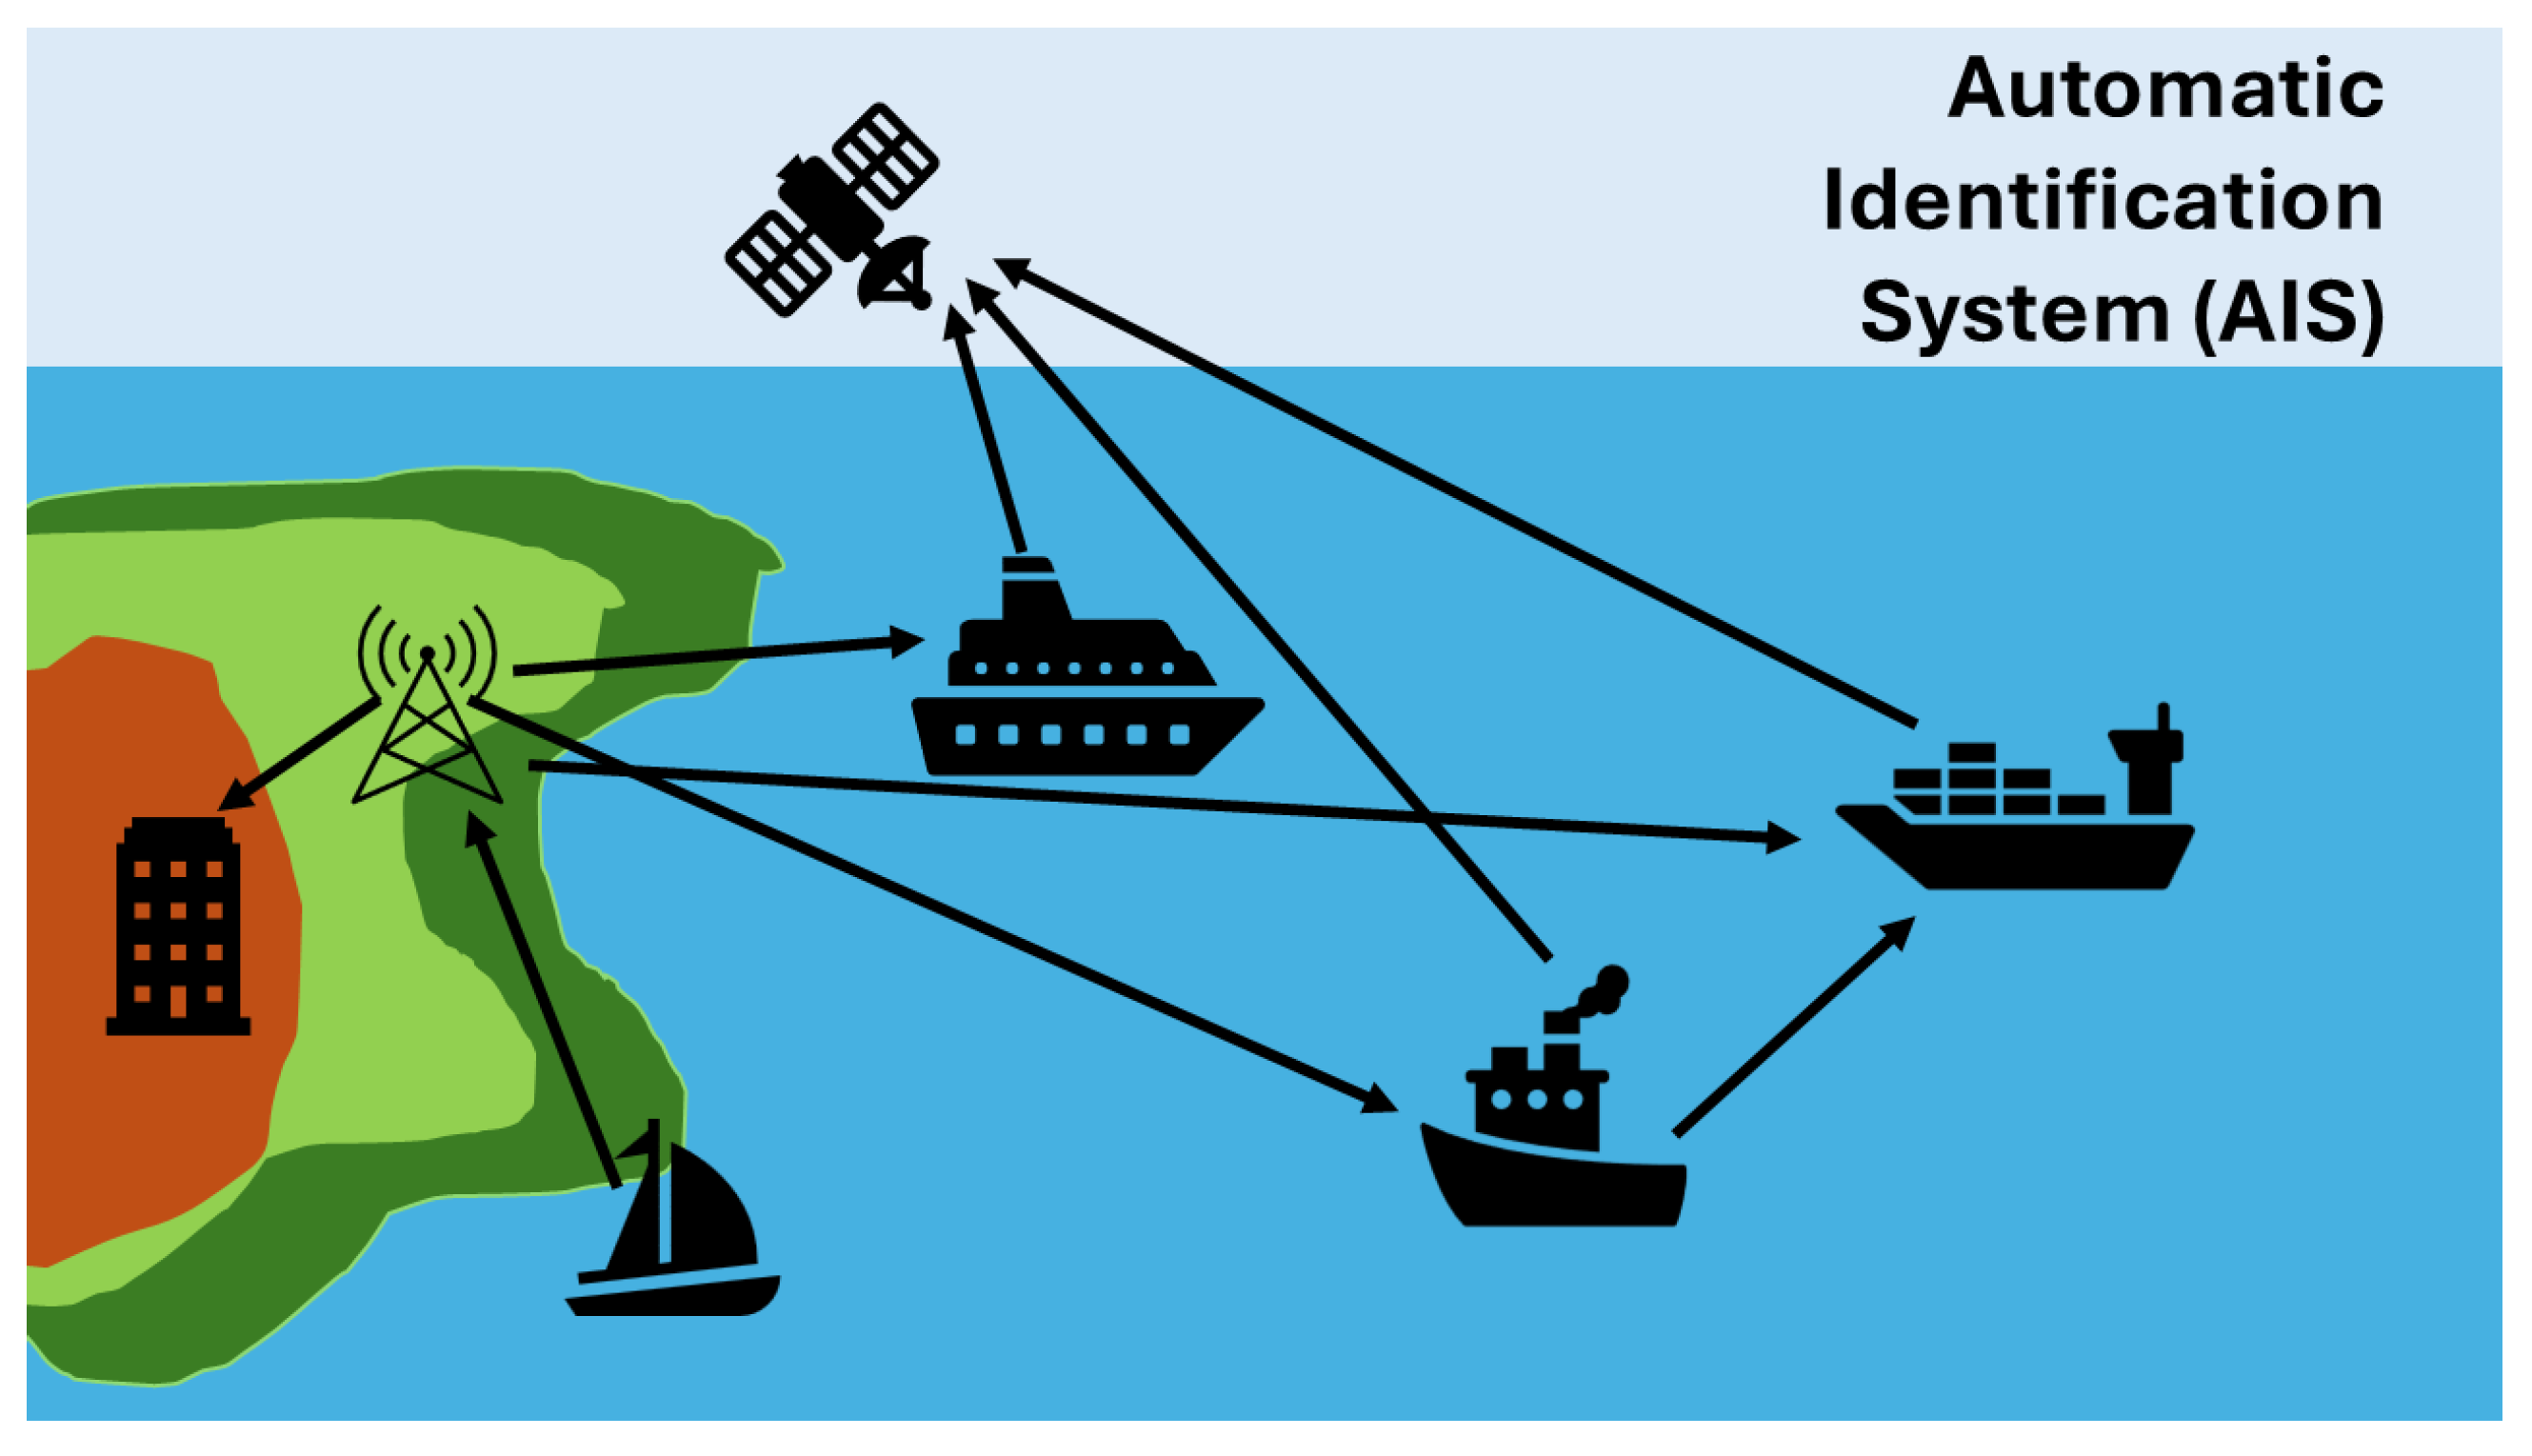
\includegraphics[scale=1]{Chapter1/Figures/ais.jpeg}	
	\caption{\glsentryshort{ais} System used in Maritime Surveillance }
	\label{fig:universe}
\end{figure}


\section[Literature Review]{\textbf{Literature Review}}

Maritime surveillance is one area where the last few years have seen a surge of research activity due to the increasing inadequacy of traditional methods of maritime surveillance and the rapid maturation of deep learning and computer vision technologies. The literature reviewed covers ship detection architecture, multi-object tracking algorithm, adverse-condition robustness, and identification of gaps that drive the proposed integrated system. The next paragraphs sum up the main findings and limitations of the respective works reviewed.

Hao et al.~\cite{Hao2025} suggested a light multi-object ship tracking algorithm, which uses an enhanced YOLOv7tiny detection backbone coupled with a StrongSORT based tracking backbone augmented by trajectory association techniques. The experiment has shown better detection accuracy with much smaller model size, which is appropriate in terms of resource constraints of the hardware. The trajectory association further minimized errors on identity switching as opposed to standard tracking baselines. The use of YOLOv7tiny instead of the more recent \gls{yolov8} architecture also limits the possible detection performance and the system has less robustness to situations where there is severe occlusion between closely clustered vessels.

Zhang et al.~\cite{Zhang2024Survey} provided a detailed review of the convolutional and transformer-based solutions to visual ship detection and tracking, synthesising the development of convolutional and transformer-based image processing across different maritime scenarios. The paper has identified key issues that keep reoccurring throughout the literature and these included: occlusion, highly variable ship scales across the ranges of detection and performance degradation in harsh weather conditions, such as, fog, rain and low light conditions. Although the survey does give a good understanding of the state of the art, it does not suggest an original integrated solution or real-time implementation, which limits its direct applicability as a deployable solution.

Li and Wang.\cite{Li2024} created EGM-\gls{yolov8}, a lightweight version of the \gls{yolov8} detection model with an efficient feature fusion module and channel attention mechanism specifically designed to detect maritime ships. The model also attained a 13.57\% reduction of parameters relative to the standard \gls{yolov8} baseline and at the same time, it is also able to achieve a greater recall across test scenarios hence demonstrating excellent real-time performance suitable on resource limited surveillance platforms. Although these contributions are made, the work is about the detection in isolation - no tracking and trajectory prediction module is included, and the utility of the system is limited to the single-frame localization, but without the tracking and trajectory prediction module, and without the behavioural analytics.

Jian et al.~\cite{Jian2024} developed a maritime ship target detection study, through an optimization of the \gls{yolov8} model, which has been trained on a large scale dataset of over 80 thousand annotated maritime images, with a diverse range of sea conditions, vessel orientation and environmental factors. The paper found that performance on complex sea scenes was significantly enhanced by large-scale domain-specific training data, over baselines not optimised. Nevertheless, the work is limited to detection, but no one thinks about the multi-frame tracking, identity preservation, or movement prediction. The optimization cost of the optimized model is also reported to be more than the lightweight alternatives, a factor that is also of concern when it comes to the implementation of the optimized model in real-time embedded systems. 

Ma et al.~\cite{Ma2024} suggested DeepSORT-OCR a ship tracking system based on DeepSORT, which adds an Optical Character Recognition (OCR) module that could read hull identification numbers on the imagery of the vessels. The system was able to recognize Multi-Object Tracking Accuracy (MOTA) of 77.18\% and show a much higher identity consistency compared to appearance-only tracking baselines. In spite of these advantages, the scheme has a very serious operational disadvantage, namely, it must have visible hull numbers, and it must have high-resolution camera images, which makes the scheme unworkable in long-range surveillance scenarios, or in situations where hull marks are obscured by weather, distance, or the angle of the camera. 

Yuan et al.~\cite{Yuan2024} created RT-FogNet, a real-time ship detection model that is specifically designed to operate under low visibility conditions in the maritime system, such as fog, backlight, and water surface reflections in the inland waterways. The model utilises a lightweight platform that is optimised to run on realistic waterway infrastructure, and can deliver reliable detection performance under less than ideal illumination conditions under which conventional detectors fail. Although RT-FogNet is a significant step towards robustness to environmental degradation, the system is designed to work only in the inland waterway settings with only one object to be tracked, and does not address the open-sea multi-object tracking, vessel identity management or predictive path modeling.

\subsection{Review of Literature}
The literature surveyed for this project spans four key domains: ship detection using deep learning architectures, multi-object tracking algorithms for maritime environments, trajectory prediction using time-series models, and robustness under adverse maritime conditions. The reviewed works collectively highlight the evolution of AI-driven surveillance techniques and reveal critical gaps in existing systems, particularly the absence of integrated end-to-end pipelines combining detection, tracking, and predictive modeling.

\subsubsection{\textbf{Ship Detection in Maritime Environments}}

Recent research has demonstrated significant progress in applying convolutional neural network-based detectors to maritime ship detection. Li and Wang \parencite{Li2025} proposed EGM-\gls{yolov8}, a lightweight variant of \gls{yolov8} enhanced with efficient feature fusion and channel attention mechanisms, achieving a 13.57\% reduction in model parameters while improving recall for maritime ship detection. Jian et al. \parencite{Jian2025} developed an optimized \gls{yolov8} model trained on a large-scale dataset of over 80,000 annotated maritime images, demonstrating improved detection accuracy across complex sea scenes with varying vessel orientations and environmental conditions. Yuan et al. \parencite{Yuan2026} introduced RT-FogNet, a real-time detection model specifically engineered for low-visibility inland waterway conditions including fog, backlight, and water surface reflections, achieving reliable detection under adverse illumination where conventional detectors fail.

\subsubsection{\textbf{Multi-Object Tracking for Vessel Monitoring}}

The consistent tracking of multiple vessels across dynamic video frames presents unique challenges in maritime environments, including occlusion, re-entry, and cluttered backgrounds. Hao et al. \parencite{Hao2025} proposed a lightweight multi-object ship tracking algorithm combining an improved YOLOv7tiny backbone with StrongSORT-based tracking and trajectory association, reducing identity switching errors and demonstrating suitability for real-time maritime use on resource-constrained hardware. Ma et al. \parencite{Ma2026} presented DeepSORT-OCR, which augments the standard DeepSORT tracker with an OCR module for hull number recognition, achieving a Multi-Object Tracking Accuracy (MOTA) of 77.18\% with stronger identity consistency compared to appearance-only tracking baselines. Zhang et al. \parencite{Zhang2025} provided a comprehensive survey of deep learning methods for visual ship detection and tracking, cataloguing recurring challenges such as variable ship scales, occlusion, and performance degradation under harsh weather, forming a strong conceptual basis for the design of the proposed system.

\subsubsection{\textbf{Research Gaps Identified}}

A critical synthesis of the reviewed literature reveals several persistent gaps that motivate the proposed work. The majority of existing systems address only one component of the surveillance pipeline — either detection or basic tracking — without integrating both into a cohesive real-time framework. None of the reviewed works combine ship detection, identity-preserving multi-object tracking, motion parameter estimation, and future trajectory prediction within a single end-to-end system. Tracking systems dependent on hull number recognition introduce operational constraints unsustainable under real-world maritime conditions, while detection-only models provide no temporal awareness of vessel behaviour. Furthermore, predictive path modeling from video-based inputs remains largely unaddressed in the current literature. The proposed system directly addresses these gaps by integrating \gls{yolov8}-based detection, \gls{deepocsort} tracking with \gls{reid}, \gls{lstm} trajectory prediction, and geospatial visualization into a unified real-time maritime surveillance pipeline \parencite{Hao2025, Zhang2025, Li2025, Jian2025, Ma2026, Yuan2026}.

\section[Motivation]{\textbf{Motivation}}

The surveillance of the sea is one of the most severely under-serviced aspects of contemporary security and environmental surveillance even though its practical importance is immense. There are thousands of vessels in operation at the same time in vast oceanic areas, but the instruments at their disposal to keep track of them are, for the most part, archaic and unsatisfactory. Radar systems do not provide any visual context, \gls{ais} can only be scaled to the breadth of the geographic spread of actual maritime activity. What was of special interest to us in this problem was its multi-layered character--it was not sufficient to detect ships, but the system had to continually track each ship across frames, manage occlusions and reappearances, and predict future motion, all in real time, under random and unpredictable lighting and sea conditions. On top of a technical challenge, the cost of poor maritime surveillance is very tangible in terms of accidents, illegal fishing, smuggling, and border violations all come with real costs to human safety, national security and marine biodiversity. This project was both technically interesting and truly valuable, which is why it aligns with \gls{sdg} 9 (Industry, Innovation and Infrastructure) and \gls{sdg} 14 (Life Below Water).


\section[Problem statement]{\textbf{Problem statement}}

The current maritime surveillance systems, radar, \gls{ais} and manual video surveillance are all found wanting in their ability to provide vessel oversight over large maritime zones and to provide a visual context, to be dependent on vessel compliance and to scale to large maritime areas. None of these methods can identify multiple vessels simultaneously, have identities consistent across dynamic video frames or predict future trajectories and authorities can always be reactive. The environmental issues like different sources of illumination, reflections by water, and occlusiveness also worsen their reliability. Consequently, there is an urgent requirement of an automated, vision-based intelligent system that can be able to detect multiple ships in real-time, conduct persistent identity-preserving tracking, and predictive path modeling to allow it to perform proactive maritime surveillance and make informed decisions across the coastal security, port management, and marine ecosystem protection.


\section[Objectives]{\textbf{Objectives}}
The objectives of the project are
\begin{enumerate}
\item To develop an intelligent maritime surveillance system capable of detecting and tracking multiple ships in real-time using \gls{yolov8} for accurate ship detection and \gls{deepocsort} for maintaining consistent vessel identities across frames, robust against real-world maritime challenges such as occlusion, lighting variations, and water surface reflections.
\item To extract trajectory information from tracked vessels and apply predictive models specifically \gls{lstm} networks and Kalman Filters to forecast future ship paths, enabling proactive monitoring and early detection of anomalous vessel behaviour.
\item To design an integrated visualization system that displays detection results, unique tracking identifiers, movement trajectories, predicted paths, and geospatial vessel positions, providing a comprehensive real-time situational awareness interface for maritime surveillance applications.
\end{enumerate}


\section[Brief Methodology of the project]{\textbf{Brief Methodology of the project}}
The system proposed has a modular pipelined architecture in which each stage processes and sends data to the next, making it scalable and able to perform in real time. Maritime video ingestion initiates the methodology that involves the extraction and preprocessing of raw frames into model input. Every frame is processed through a \gls{yolov8} detection model to detect and localize all ships using a bounding box regression model. Detected ships are then inputted into the \gls{deepocsort} multi-object tracking module which assigns and maintains unique identities across frames by appearance-based \gls{reid} and Kalman filter state estimation. Over time centroid coordinates of tracked vessels are recorded and trajectory sequences of the tracked vessel built by centroid coordinates and motion parameters, such as speed, heading, and cardinal direction, are derived analytically using inter-frame displacement. These paths-sequences are then used by an \gls{lstm} neural network to predict the future vessel positions. Lastly, all outputs (bounding boxes, tracking IDs, motion vectors and predicted paths), are displayed on the video feed and geospatially mapped with Folium, to provide a single real-time interface of maritime monitoring.


\section[Assumptions made / Constraints of the project]{\textbf{Assumptions made / Constraints of the project}}

The system is planned, and tested on the following assumptions. Input is presumed to be video footage captured by a fixed camera in one location; a coastal watchtower or a port surveillance unit. It is assumed that ships are sufficiently visible and distinguishable to the water background and that the \gls{yolov8} model has been trained on a representative maritime dataset that covers the variations in ship size, type and environmental conditions. The movement of vessels is also assumed to be governed by time-invariant trajectories since sharp manoeuvres can decrease the prediction accuracy of \glspl{lstm}. It is also assumed that a computing environment with a graphics card is available since real-time throughput cannot be assured on hardware without graphics cards.
As follows, the constraints control the extent and legitimacy of the project. The system only accepts video as an input and does not take radar or \gls{ais} data. The performance of detection and tracking can diminish when the weather is extreme, i.e. when the visibility is low and the rain is heavy. The accuracy of prediction of \gls{lstm} is limited by the length and quality of data available on the historical trajectory of a given vessel, as well as the fact that the accuracy of prediction decreases with longer and lower quality data available on the historical trajectory of a given vessel. Single-feed surveillance is the only type that is currently supported by the system, and it does not accept several simultaneous camera feeds. The accuracy of geospatial mapping process also requires accurate camera calibration parameters to ensure accurate pixel to coordinate mapping.


\section[Organization of the Report]{\textbf{Organization of the Report}}

This report is organized as follows.
\begin{itemize}
\item Chapter 2 discusses the review of existing literature on maritime surveillance systems, covering ship detection, multi-object tracking, and trajectory prediction methods, along with identified research gaps that motivate the proposed system.
\item Chapter 3 discusses the system design and methodology, elaborating the modular pipeline architecture encompassing video ingestion, \gls{yolov8}-based detection, \gls{deepocsort} tracking, motion parameter estimation, \gls{lstm} trajectory prediction, and geospatial visualization.
\item Chapter 4 discusses the implementation details of each module, including dataset preparation, model training procedures, integration of the prediction pipeline, and the tools and frameworks employed for development.
\item Chapter 5 discusses the experimental results and performance evaluation of the system, presenting detection accuracy, tracking consistency, trajectory prediction outcomes, and qualitative visualization outputs across various maritime test scenarios.
\item Chapter 6 discusses the conclusions drawn from the project, highlighting key contributions, limitations of the current system, and potential directions for future enhancement and real-world deployment.
\end{itemize}